% As a demonstration that our entire strong lens program pipeline -- from discovery to high resolution and spectroscopic confirmation and lensing modeling is ready, we show the modeling of one system.

As a demonstration, we use \gigal \citep{gu2022a} to model one lens system observed by our DESI and Keck NIRES programs, \href{https://www.legacysurvey.org/viewer/?ra=165.4753&dec=-6.0424&layer=ls-dr9&pixscale=0.262&zoom=16}{DESI-165.4754-06.0423}.
The modeling of other systems with \hst data will be presented in future publications.
DESI-165.4754-06.0423 was discovered in H21, with a numerical grade of 2.5 (out of 4), corresponding to a C~grade 
(In H21, we mentioned that all candidates with a human inspection score $\geq 2.5$ are likely lensing systems).
%The photometric redshift for the lens is 0.447$\pm$0.074 \citep{zhou2020a}.
The lens and source redshifts of $z_d = 0.4834$ and
$z_s = 1.6748$ are obtained from DESI and Keck NIRES, respectively (Paper II \& III).
Based on color and photo-$z$, 
this galaxy appears to be at the center, 
and the brightest member (18.8~mag in $r$-band), of a small group.
While most other group members are 12$\twopr$ or more away, 
there is a small nearby galaxy with $z_{phot} = 0.579\pm 0.166$, consistent with it being a group member, 
with a $r$-band magnitude of 23.2~mag.
We will refer to this object as the ``nearby galaxy''.
% The lens and source redshifts are $z_d = 0.483$ (DESI) and
% $z_s = 1.6748$ (Keck NIRES), with several prominent emission lines 
% The source spectroscopic redshift was obtained on Keck NIRES, 
% (H-$\alpha$, \ion{N}{2}, [\ion{O}{3}], and H-$\beta$) identified (Paper~II, in prep). 
The Legacy Surveys image of DESI-165.4754-06.0423 shows an elliptical galaxy surrounded by what appears to be an almost complete Einstein ring, with an Einstein radius of approximately $\sim 2.5''$.
The \hst image showed that it is a quadruply lensed system. 



\gigal is a fully forward-modeling Bayesian lens modeling pipeline.
Briefly, it consists of three steps: finding the maximum a posteriori (MAP) for the lensing parameters via multi-start gradient descent, determining a surrogate multidimensional Gaussian covariance matrix for these parameters using stochastic variational inference (SVI), and finally sampling with Hamiltonian Monte Carlo (HMC).
All three steps use gradient descent with automatic differentiation and take advantage of GPU acceleration.  
Unlike with other lens modeling pipelines, 
we do not take a staged approach, 
which may first fit for and then subtract the lens light, 
followed by initializing with a simple model and gradually increasing the model complexity, typically fixing the values of some parameters in this process (e.g., \ser index values).
% \citep[e.g.,][]{shajib2021a, etherington2022a}.
Instead, to avoid landing in a local minimum and to account for full statistical uncertainties, we perform full forward modeling.
It is robust and very fast (\ed{$\sim 3$~hours even for a challenging system such as this one, as we will show below).}
% Previously using ground-based data, we successfully applied GIGA-Lens to a real lens system for the first time, 
% DESI-253.2534+26.8843 \citep{cikota2023a}.


 
%%%% do not remove
% https://docs.google.com/presentation/d/1u7x5Xe9K2XOj3UoUcJ83hy-OS4bQcMoTTvQ2L_5JYtA/edit#slide=id.g25d2fdac01b_0_57

% The \hst images are drizzled to $0.065\twopr$.
We show this system in Figure~\ref{fig:what-to-mask} again, 
although with a different orientation from Figure~\ref{fig:hstpanel-2}.
% We use a 27$\times$27 pixel empirical \textcolor{red}{PSF extracted by 
% Lenstronomy \citep{birrer2021a}}.
We use a $27 \times 27$ pixel empirical PSF generated by stacking PSF-like objects identified by SExtractor.\footnote{We use the implementation provided in \url{https://github.com/sibirrer/AstroObjectAnalyser/}.}
Our mass model comprises an elliptical power law (EPL) for the main lens with external shear.
\ed{The EPL model is characterized by the surface mass density expressed in units of the critical density, commonly referred to as convergence,
\begin{equation}
    \kappa(x_{lens}, y_{lens}) = \frac{3-\gamma}{2}\left(\frac{\theta_E}{\sqrt{q x_{lens}^2+y_{lens}^2 / q}}\right)^{\gamma-1},
\end{equation}
where $\theta_E$ is the Einstein radius (in the intermediate-axis convention), $\gamma$ is the deprojected 3D mass profile slope \citep[e.g.,][]{tessore2015a}, $(x_{lens}, y_{lens})$ are lens-centric coordinates, and $q$ is the axial ratio.
In lens modeling, often $q$ and the position angle $\phi$ are reparametrized as eccentricities,
\begin{equation}
    (\epsilon_1, \epsilon_2) = \frac{1-q}{1+q}\left(cos(2\phi), sin(2\phi)\right).
\end{equation}
The external shear is characterized by $\gamma_{ext, 1}$ and $\gamma_{ext, 2}$.}
%The deflection angle can be calculated iteratively using the Gaussian hypergeometric function, reaching a truncation error $\lesssim 10^{-16}$ within $35$ iterations for $q\gtrsim 0.5$ \citep{tessore2015a}.




%We include an external shear characterized by a deflection angle, where $(x,y)$ are image coordinates:
%\begin{equation}
%    \alpha_{ext}(x,y)=\left(\gamma_{ext, 1}x+\gamma_{ext, 2}y, \gamma_{ext, 2}x-\gamma_{ext, 1}y\right).
%\end{equation}

%while the external shear is characterized by $\gamma_{ext, 1}, \gamma_{ext, 2}$.

We model the lens light with two elliptical \ser profiles\ed{,
%The elliptical \ser profile is defined as,
defined as,
\begin{equation}
I(x_{light}, y_{light})= I_0 \ exp\left(-b_n\left(\left(\frac{\sqrt{q x_{light}^2+y_{light}^2 / q}}{R}\right)^{1/n} - 1
\right)
\right),
\end{equation}
where $b_n = 1.9992 n - 0.3271$, $n$ is the \ser index, $(x_{light}, y_{light})$ are light coordinates, and $R$ is the half-light radius. In the modeling process, we again use the eccentricities as parameters instead of $q$ and the position angle $\phi$.}
We additionally model the light of the small nearby galaxy,
\ed{which also appears to be an elliptical galaxy, based on its color and morphology,} again using two elliptical \ser profiles.
\ed{Since the central regions of an elliptical galaxy are not always modeled well by \ser profiles \citep[e.g.,][]{shajib2021a}, a circular area with a radius of 2.5 pixels at its center (Figure~\ref{fig:what-to-mask}, dashed arrow) is masked.}
We do not model its mass.
We model the source using an elliptical \ser profile and \ed{shapelets} with $n_{max} = 6$ \citep{birrer2015a}.
We mask out the light for three very faint galaxies only visible in the \hst image (blue circles in Figure~\ref{fig:what-to-mask}).
We also mask out the small object embedded (in projection) in arc A (Figure~\ref{fig:what-to-mask}, solid arrow).\footnote{
We find that whether to include a mass model for this object \ed{makes} negligible difference for the main lens parameters, which is the goal of this modeling effort.
Determining whether it is a galaxy or a MW star may have implications for testing the detection of small perturbers in lensing \citep[e.g.,][]{vegetti2010a} but this is out of scope for this work and will be left to a future investigation.}
Our model consists of \nparams parameters, defined in Table~\ref{tab:parameters}. 

\clearpage
% This is a fully forward-modeling Bayesian approach.
% Need to mention VDISP from DESI, from fastspecfit.
% Mention dynamical mass from DESI.}

% Introduce EPL+Sersic

\begin{minipage}{\linewidth}
%\vspace{5pt}
\makebox[\linewidth]{
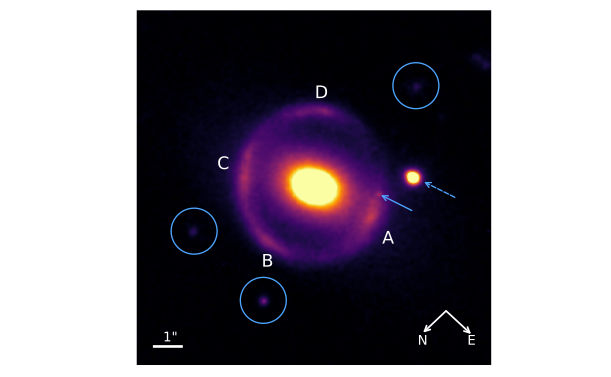
\includegraphics[keepaspectratio=true,scale=0.75]{figs/observed_img_v2.png}}
\captionof{figure}{
DESI-165.4754-06.0423 in \hst WFC3 F140W.
 The four lensed images are labeled clockwise as A, B, C and D.
 To model this system, we mask out the light from three faint objects (circles) and the small object (solid arrow) in arc A (in projection).
 We also mask out the central region of the small nearby galaxy with a circular mask of radius 2.5 pixel (dashed arrow).}
\label{fig:what-to-mask}
%\vspace{-5pt}
\end{minipage}




% {\color{red} 
% Finally we model the light, but not the mass, of a nearby galaxy (dashed arrow in Figure~\ref{fig:what-to-mask}), 
% masking a small circular region (with a diameter of xx pixels) near the center.}

\begin{table}
\caption{Prior distribution used for lens modeling}
\begin{align*}
\text{Lens mass:} &
\begin{cases}
    \hfill \theta_E & \sim \exp\left(\mathcal{N}(\ln 2.5, 0.25\right) \\[1pt]
    \hfill \gamma & \sim \mathcal{TN}\left(2, 0.25, 1, 2.7\right) \\[1pt]
    \hfill \epsilon_{1}, \epsilon_{2} & \sim \mathcal{N}(0, 0.1) \\[1pt]
    \hfill x, y & \sim \mathcal{N}(0, 0.05) \\[1pt]
    \hfill \gamma_{ext, 1}, \gamma_{ext, 2} & \sim \mathcal{N}(0, 0.05)
\end{cases} \\
\text{Lens light:} &
\begin{cases}
    \hfill R_{\text{l}} & \ed{\sim \exp(\mathcal{N}(\ln 1, 0.15)) / \exp(\mathcal{N}({\ln 1, 0.15}))} \\[1pt]
    \hfill n_{\text{l}} & \ed{\sim \mathcal{U}(0.5, 10)/ \mathcal{U}(0.5, 10 )} \\[1pt]
    \hfill \epsilon_{\text{l},1}, \epsilon_{\text{l},2} & \ed{\sim \mathcal{N}(0, 0.15) / \mathcal{N}(0, 0.15)} \\[1pt]
    \hfill x_{\text{l}} & \ed{\sim \mathcal{N}(0, 0.05) / \mathcal{N}(0, 0.10)} \\[1pt]
    \hfill y_{\text{l}} & \ed{\sim \mathcal{N}(0, 0.05) / \mathcal{N}(0, 0.10)}
\end{cases} \\
\text{Source light:} &
\begin{cases}
    \hfill R_{\text{s}} & \sim \exp\left(\mathcal{N}(\ln 0.25, 0.15\right)) \\[1pt]
    \hfill n_{\text{s}} & \sim \mathcal{U}(0.5, 6) \\[1pt]
    \hfill \epsilon_{\text{s},1}, \epsilon_{\text{s},2} & \sim \mathcal{N}(0, 0.15) \\[1pt]
    \hfill x_{\text{s}}, y_{\text{s}} & \sim \mathcal{N}(0, 0.1) \\[1pt]
    \hfill \beta_{shp} & \sim \exp (\mathcal{N}(\ln 0.1, 0.1)) \\[1pt]
    \hfill x_{shp}, y_{shp} & \sim \mathcal{N}(0, 0.05)
\end{cases} \\
\text{Nearby galaxy:} &
\begin{cases}
    \hfill R_{\text{g}} & \ed{\sim \exp(\mathcal{N}(\ln 0.4, 0.2)) / \exp(\mathcal{N}({\ln 0.4, 0.2} ))} \\[1pt]
    \hfill n_{\text{g}} & \ed{\sim \mathcal{U}(0.5, 5)/\mathcal{U} (0.5, 5)} \\[1pt]
    \hfill \epsilon_{\text{g},1}, \epsilon_{\text{g},2} & \ed{\sim \mathcal{TN}\left(0, 0.15, -0.3, 0.3\right) / \mathcal{TN}\left(0, 0.15, -0.3, 0.3 \right)} \\[1pt]
    \hfill x_{\text{g}} & \ed{\sim \mathcal{TN}(3.7, 0.05, 3.55, 3.85) / \mathcal{TN}(3.7, 0.05, 3.55, 3.85)} \\[1pt]
    \hfill y_{\text{g}} & \ed{\sim \mathcal{TN}(0.25, 0.05, 0.1, 0.4) /\mathcal{TN}(0.25, 0.05, 0.1, 0.4)}
\end{cases}
\end{align*}
\label{tab:parameters}
{\small Notes --- 
%\tablecomments{
The mass model consists of EPL for the lens mass profile and external shear ($\gamma_{ext}$). 
$\theta_E$ is the Einstein radius in arcsec, while $\gamma$ defines the slope of the EPL profile.
$x$ and $y$ are the mass center coordinates of the lens. %in arcsec, 
$\gamma_{1, \text{ext}}$ \ed{and $\gamma_{2, \text{ext}}$} are the external shear components.
The parameters $\epsilon_1$ and $\epsilon_2$ are the lens mass eccentricities.
For the light model, subscripts $l$, $s$, $g$ indicate parameters belonging to the light profiles of the lens, the source, and the nearby galaxy, respectively. 
Thus $(\epsilon_{l,1}$, $\epsilon_{l,2})$, $(\epsilon_{s,1}$, $\epsilon_{s,2})$, $(\epsilon_{g,1}$, $\epsilon_{g,2})$ are the lens, source, and nearby galaxy light eccentricities, respectively.
For the light of the lens and the nearby galaxy, we use two elliptical S{\'e}rsic profiles each, with their prior distributions separated with a slash.
$R_l$, $R_s, R_g$ are the half-light radii, and $n_l$, $n_s, n_g$ are the S{\'e}rsic indices for the respective objects. 
$(x_l, y_l)$, $(x_s, y_s)$, $(x_g, y_g)$ describe their centers. 
The subscript $shp$ refers to the shapelets component for 
% profile used for 
the source.
Finally, $\mathcal{U}(a, b)$ indicates a uniform distribution with support $[a, b]$, $\mathcal{N}(\mu, \sigma)$ is a Gaussian with mean $\mu$ and standard deviation $\sigma$, and $\mathcal{TN}(\mu, \sigma, a, b)$ is a truncated Gaussian with support $[a, b]$.}
%\ed{For the light profiles of the lens and the nearby galaxy, we use two \ser models for each, with identical prior values. Both sets of priors for each galaxy are shown with a slash separating them.}}
\end{table}

We achieve excellent \ed{residuals} (Figure~\ref{fig:model}). 
The best-fit parameters are shown in \ed{Tables~\ref{tab:best-fit-params} and \ref{tab:best-fit-light-params}}.
% representative 
The sampling results for the lens and external shear mass parameters are shown in Figure~\ref{fig:cornerplot}. 
For this system, the marginal distributions of the SVI posterior match the HMC sampling results for some parameter pairs as well as they do for the simulated systems presented in \citet[][their Figures~6 and A2]{gu2022a}, although the match is not as close for all pairs. Overall, the SVI posterior provides a good approximation to the HMC samples, demonstrating the efficacy of the SVI step.
%%%%(the full corner plot for all \nparams model parameters is provided in the Appendix). \textcolor{red}{Change if the full corner plot is not shown}
We determine the Einstein radius of the lens to be $\theta_E = \thetaEfit$ 
and the slope of the power law mass profile to be $\gamma = \gammafit$.
The total mass within the critical curve is $1.7390_{-0.0043}^{+0.0046} \times 10^{12} \, M_{\odot}$. 
We use the larger $R_e$ from the two \ser models as the effective light radius for the lensing galaxy, \Refit, or \Refitkpc, \ed{adopting the cosmological parameters from \citet{planck2020a}: $H_0$ = 67.4 $\pm$ 0.5 km s$^{-1}$ Mpc$^{-1}$, $\Omega _{\Lambda}$ = 0.6847 $\pm$ 0.0073, and $\Omega _{M}$ = 0.315 $\pm$ 0.007}.
The best-fit model predicts magnifications of 
$25.0\pm 1.6$, $59.0\pm 1.6$, $51.1\pm 2.7$, and $35.43\pm 0.79$ for images A, B, C, and D, respectively (Figure~\ref{fig:what-to-mask}), computed as the average of the first and second methods in Appendix~\ref{sec:append-mag}.

As a further analysis on our best-fit $\gamma$, 
\ed{we explore regions higher than the prior for $\gamma$ in Table~\ref{tab:parameters} ($\mathcal{TN}(2,0.25,1,2.7)$) and demonstrate stability in the other parameters and the consistent tendency for $\gamma$ to approach the lower boundary.
We 
% modeled the system using 
use two other priors for $\gamma$, while for all other parameters the prior remains unchanged.
}
% to restrict the limits for $\gamma$. 
% The prior for all other parameters remained unchanged.
One is a truncated Gaussian distribution centered around $2.0$ with boundaries at $1.5$ and $2.5$.
For the second, we use a uniform prior between $2.0$ and $3.0$.
In both cases, the corner plot shows consistent values with our best-fit model for all parameters except for $\gamma$, whose posterior is pushing against the lower boundary, $1.5$ and $2.0$, respectively. In addition, we observe a $42.13 \ \chi^2$ improvement for using the prior with the $1.5$ lower bound and a $551.87 \ \chi^2$ improvement for using the prior with the $2.0$ lower bound, favoring our best-fit model in both cases.

%\textcolor{red}{$-2.31$, 4.52, $-4.79$, and 3.34} (\ed{also, say these values are from which method in the Appendix?})

% The highest being for image C. 
%%%% DO NOT DELETE!
%As for time delays, the first image to be formed was image D. Next, image B is predicted to have appeared after 12.67 days, followed by image C, after 20.19 days. The last arc to be formed was image A, with a delay of 42.38 days. All time delays are relative to image D.


\begin{minipage}{\linewidth}
\vspace{5pt}
\makebox[\linewidth]{
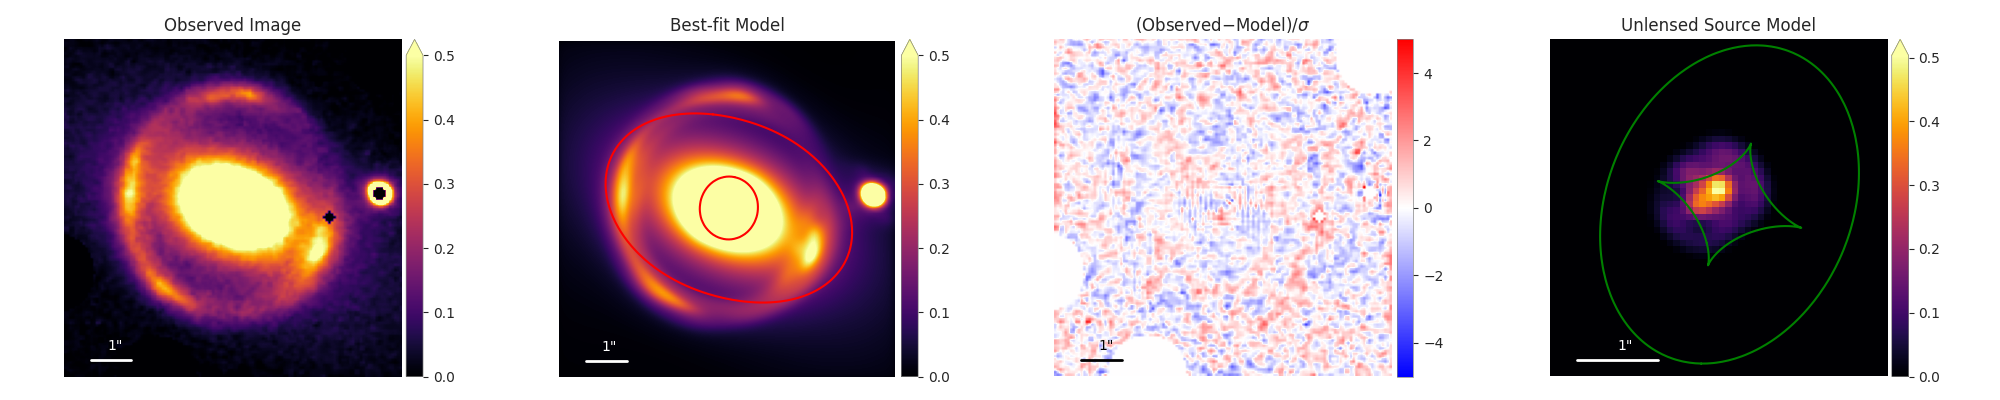
\includegraphics[keepaspectratio=true,scale=0.40]{figs/model-residual-HMC-zoom2.png}}
% Before: model_residual_inferno
\captionof{figure}{From left to right, we show:
the observed \hst image (same orientation as in Figure \ref{fig:what-to-mask}), 
our best-fit model with critical curves in red, 
the reduced residual map,
and the reconstruction of the unlensed source with caustics in green. Notice the presence of an inner critical curve and caustic due to the fact that $\gamma<2$.
}
\label{fig:model}
\vspace{5pt}
\end{minipage}





Our sampling results are robust and statistically consistent using two widely employed metrics to measure the degree of convergence: 
the potential scale reduction factor (PSRF), \ed{often represented as \rhat} \citep{gelman1992a}, and the effective sample size (ESS). \ed{In cosmological studies, these two criteria have been widely adopted \citep[e.g.,][]{krolewski2021a, douspis2022a, mandel2022a, rubin2023a}.}
An $\hat{R}$ that is close to 1 and a large ESS indicate that convergence to the same stationary distribution has been achieved. 
 % (e.g., \textcolor{red}{see Figure xx -- traces for $\gamma$}).
%it is suggested that 
\citet{gelman1992a} suggested that an appropriate condition is $\hat{R} < 1.2$.\footnote{Quoting from the \href{https://www.tensorflow.org/probability/api_docs/python/tfp/mcmc/potential_scale_reduction}{TensorFlow documentation}, ``Sometimes, $\rhat < 1.2$ is used to indicate approximate convergence." This implementation by TensorFlow, which we use, is approximately the square of the more recent (re)definition of \rhat---thus, using this definition, the equivalent threshold would be $\rhat < 1.1$ \citep{gelman2014a}.\label{fn:rhat}}

% \citep[see also][]{gelman2014a}.
%\footnote{See also Chap.\ 36 of the latest version of \href{https://mc-stan.org/docs/2_33/stan-users-guide-2_33.pdf}{the Stan User's Guide.}}  

%\footnote{For these two metrics, 
%see also   
%TensorFlow documentation for \href{https://www.tensorflow.org/probability/api_docs/python/tfp/mcmc/potential_scale_reduction}{$\hat{R}$} and \href{https://www.tensorflow.org/probability/api_docs/python/tfp/mcmc/effective_sample_size}{effective sample size.}}
% For our best-fit model, the \rhat values for all mass and light parameters of the lens and for all light parameters of the source are below 1.03.
% For the nearby galaxy light parameters, all except for two, $n_{\text{g}}$ and $\epsilon_{\text{g},1}$ (with \rhat = 1.12 and 1.10, respectively),
% \rhat is less than 1.1.
% While these two parameters are at or slightly above the threshold, 
% all parameters of interest \citep[][Chap.\ 11]{gelman2014a}, 
% especially the mass parameters of the lens and the light parameters of the source, are well below the threshold.
For our best-fit model, the \rhat values for all mass and light parameters of the lens and for all light parameters of the source are below 1.10. For the nearby galaxy light parameters, \rhat is less than 1.12 and thus, all parameters are well below the threshold of $\rhat < 1.2$.
% For our best-fit model, the \rhat values for all mass and light parameters of the lens and for all light parameters of the source are below 1.03. For the nearby galaxy light parameters, \rhat is less than 1.12. Hence, all parameters, especially the mass parameters of the lens and the light parameters of the source, are well below the threshold.
As for ESS, $\mathcal{O}(10^3)$ is considered sufficiently high \citep[e.g.,][]{carpenter2017a, mandel2022a}. For our best-fit model, the minimum is 32,200, and the maximum, 40,000, demonstrating excellent sampling efficiency with very low autocorrelation \citep[see, e.g.,][]{gu2022a}. 
% If we leave out the second galaxy light parameters, the minimum ESS is 37,000.

In addition to being robust, our modeling approach is also fast.
On a GPU node on the {\it Perlmutter} supercomputer at \ed{the National Energy Research Scientific Computing Center (NERSC)},\footnote{\url{https://www.nersc.gov/}} 
which has four A100 GPUs,
the total execution time is 3 hrs.\ and 13 min. (193 min.), 
with the MAP, SVI, and HMC steps taking 1 hr.\ 9 min. (69 min.), 1 hr.\ 52 min. (112 min.), and 12 min., respectively.
Considering that we take a fully forward modeling Bayesian approach with 41 model parameters for a highly nonlinear problem, 
this is remarkably fast.

\clearpage
% \FloatBarrier
\begin{deluxetable*}{lccccccc}
\tabletypesize{\scriptsize}
\tablecaption{Best-fit mass parameters for DESI-165.4754-06.0423.
%for the lens mass profile and the external shear.
\label{tab:best-fit-params}}
\renewcommand{\arraystretch}{1.4}
\tablehead{
    \colhead{$\theta_E$} &
    \colhead{$\gamma$} &
    \colhead{$\epsilon_1$} &
    \colhead{$\epsilon_2$} &
    \colhead{$x$} &
    \colhead{$y$} &
    \colhead{$\gamma_{ext, 1}$} &
    \colhead{$\gamma_{ext, 2}$} 
}
\startdata
$2.6463_{-0.0016}^{+0.0017}$& 
$1.372_{-0.022}^{+0.023}$&	
$0.1091_{-0.0020}^{+0.0020}$&$-0.1320_{-0.0020}^{+0.0020}$  & 
$0.0272_{-0.0022}^{+0.0023}$&	$-0.0018_{-0.0017}^{+0.0017}$ &
$0.0657_{-0.0024}^{+0.0024}$&	
$-0.0939_{-0.0022}^{+0.0022}$ \\
\enddata
\end{deluxetable*}
%\vspace{-15pt}


\begin{deluxetable}{l|rr|r|rr}
\tablecaption{Best-fit light parameters for DESI-\ed{165.4754-06.0423.}
\label{tab:best-fit-light-params}
}
\renewcommand{\arraystretch}{1.4}
\setlength{\tabcolsep}{10pt}
\tablehead{
    \colhead{Parameter} & \multicolumn{2}{c}{Lens light} & \colhead{Source light} & \multicolumn{2}{c}{Nearby galaxy light} 
}
\startdata
$\bm{R_e}$ &
$0.4327_{-0.0050}^{+0.0051},$&$1.888_{-0.017}^{+0.017}$&$0.614^{+0.038}_{-0.036}$&     $0.1353_{-0.0025}^{+0.0021},$&$0.227_{-0.065}^{+0.066}$\\[4pt]
$\bm{n}$ &               
$0.925_{-0.014}^{+0.014},$&$1.262_{-0.033}^{+0.035}$&$0.5050^{+0.0082}_{-0.0037}$&
$0.523_{-0.017}^{+0.032},$&$3.86_{-1.22}^{+0.81}$\\[4pt]
$\bm{\epsilon_{1}}$ &    
$0.1350_{-0.0022}^{+0.0020},$&$0.1452_{-0.0012}^{+0.0012}$&$-0.058^{+0.025}_{-0.026}$&
$0.0118_{-0.0089}^{+0.0087},$&$0.144_{-0.074}^{+0.059}$\\[4pt]
$\bm{\epsilon_{2}}$ &    
$-0.0577_{-0.0038}^{+0.0039},$&$-0.1832_{-0.0013}^{+0.0013}$&$0.192^{+0.023}_{-0.023}$& 
$-0.1124_{-0.0102}^{+0.0080},$&$0.264_{-0.055}^{+0.026}$\\[4pt]
$\bm{x}$ &
$0.0042_{-0.0014}^{+0.0013},$&$0.0437_{-0.0023}^{+0.0024}$&$0.137^{+0.013}_{-0.012}$& 
$3.6100_{-0.0039}^{+0.0023},$&$3.7347_{-0.0079}^{+0.0062}$\\[4pt]
$\bm{y}$ &
$0.0448_{-0.0012}^{+0.0013},$&$-0.0053_{-0.0018}^{+0.0018}$&$0.044^{+0.012}_{-0.012}$&
$0.3704_{-0.0011}^{+0.0014},$&$0.3580_{-0.0058}^{+0.0043}$\\[4pt]      
$\bm{\beta_{shp}}$ &
- & - & $0.0505_{-0.0030}^{+0.0031}$ & -  & - \\[4pt]
$\bm{x_{shp}}$ & - & - &$-0.0249_{-0.0040}^{+0.0039}$& - & - \\[4pt]
$\bm{y_{shp}}$ & - & - &$0.0354_{-0.0025}^{+0.0025}$& -  & - \\  
\enddata

\vspace{3pt}
\ed{\noindent \hspace{0.5em}{\small Notes ---
We model the light of both the lens and nearby galaxy with two elliptical Sérsic profiles each,
with the best-fit parameters shown in the second and last main columns, respectively.}}
%We model the light of both the lens and nearby galaxy with two elliptical Sérsic profiles each. The left subcolumn shows the inner component, and the right subcolumn the outer.}}
\end{deluxetable}


\begin{minipage}{\linewidth}
\makebox[\linewidth]{
  \includegraphics[keepaspectratio=true,scale=0.35]
  %{figs/mass_cornerplot.png}
  {figs/corner_vi_hmc_v2.png}}
\captionof{figure}{The corner plot showing our sampling results for the lens and external shear mass parameters\ed{,
with SVI and HMC samples shown in blue and black, respectively.}
}

\label{fig:cornerplot}
\end{minipage}


